\documentclass[12pt]{book}

\usepackage[utf8]{inputenc}
\usepackage[T1, T2A]{fontenc}
\usepackage[russian]{babel}
\usepackage{csquotes}

\usepackage{amsmath,amssymb}

\usepackage[backend=biber, style=numeric]{biblatex}
\addbibresource{thesis.bib}

\usepackage{float}
\usepackage{graphicx}

% ./pic is used for dynamically updated images -- python scripts
% write their output there
% when the image is finalized it is manually copied to ./pic/final
% and scripts can do whatever they want
\graphicspath{{./pic/final/} {./pic/}}

\setcounter{secnumdepth}{3}
\newcommand{\cov}{\mathrm{cov}}


\title{Байесовская деконволюция для эксперимента СФЕРА-2}

\author{Игорь Вайман}

\date{\today}

\begin{document}
	\maketitle
	
	\chapter{Описание эксперимента СФЕРА-2}

	Эксперимент СФЕРА-2 основан на сборе и регистрации черенковского света ШАЛ, отражённого от <<экрана>> -- ровной заснеженной поверхности льда озера Байкал. Установка представляет собой сферическое зеркало и мозаику ФЭУ, установленную вблизи фокальной поверхности. Черенковский свет ШАЛ, рассеиваясь на снегу, проходит через диафрагму установки, отражается от зеркала, и попадает на фотокатод. При попадании фотона с длиной волны в области чувствительности фотокатода с него выбиваются $1 - 10$ (уточнить) вторичных электронов, которые проходят систему динодов с разностью потенциалов между каждой парой, создавая в результате избыточный на аноде. Этот заряд стекает с анода через цепь усиления, создавая в результате напряжение на входе АЦП. Это напряжение считывается электроникой, в результате и составляя (вместе с некоторой телеметрией) экспериментальные данные.
	
	Этот набор физических процессов мы описываем в следующих предположениях:
	
	\begin{enumerate}
		\item В системе нет электронных шумов -- единственным источником шума являются фоновые фотоны (от звёздного и зодиакального света, так как эксперимент проводится в ясные безлунные ночи). Фотоны шума попадают в установку аналогично <<сигнальным>> фотонам -- после рассеяния на поверхности. Их поток можно приблизительно оценить по каталогам светимости звёзд и из моделей зодиакального света. (Ссылка на работу Энтиной)
		\item Работу ФЭУ можно эффективно описать одной <<рандомизированной>> испульсной характеристикой (РИХ). Понятие и применение РИХ будет раскрыто далее, в общем виде это случайная функция времени, описывающая отклик системы на один фотон, падающий на фотокатод. Главный источник случайности в установке СФЕРА-2 -- неопределённость числа вторичных фотонов, вылетевших с фотокатода, приводящая к неопределённости амплитуды импульса тока. Стоит отметить, что случайный характер ИХ проявляется именно на границе между режимом счёта фотонов и режимом измерения потока, поскольку поток фотонов уже слишком велик, чтобы разрешать отдельные импульсы, но недостаточно -- чтобы случайные характеристики эффективно усреднялись. Мы также предполагаем, что случайность импульсной характеристики проявлялась независимо между отдельными фотонами и между разными ФЭУ.
		\item Используя экспериментальные данные (данные, записанные АЦП, постоянную компоненту анодного тока и абсолютную калибровку ФЭУ) мы можем восстановить показания анодного тока (ссылка на работу по электронике). Неопределённость, вносимая анодной цепью, усилителем и (главным образом) дискретизацией сигнала на входе АЦП, хорошо известна и учитывается во вторую очередь.
	\end{enumerate}

	\chapter{Байесовская деконволюция}
	
	\label{chapt:bayesian-deconvolution}
	
	В этой главе будут описаны физические предпосылки и интуиции, связанные с системой регистрации отражённого черенковского света в эксперименте СФЕРА-2, затем на их основе будет строго поставлена задача статистической деконволюции и описан метод её решения в общем виде, и, наконец, разработанный метод будет применён к экспериментальным данным, полученным экспериментом СФЕРА-2.
	
	\section{Предпосылки}
	
	
	
	\section{Нотация}
	
	\textbf{TBD заменить фотоны на $\delta$-функции}
	
	Рассмотрим $N$ последовательных равновеликих временных бинов. Для простоты будем считать единицей времени длительность одного бина. Тогда мы можем задать временные бины интервалами $[i-1, i]$, $i = 1 \ldots N$. Обратим внимание, что при такой нумерации бинов эффект от фотонов, попавших в $i$-тый временной бин проявляется впервые в момент времени $i$. Обозначим число фотонов в каждом бине как $n_i$, $i = 1, \ldots, N$.

	Время прихода отдельного фотона относительно начала бина $t_{inbin} = \{ t \}$ будем описывать случайной величиной, подразумевая, что мы не интересуемся такими детальными характеристиками сигнала. Эта величина может быть, вообще говоря, распределена произвольным образом в интервале $\left[0, 1\right)$, однако мы в простейшем случае будем считать $t_{inbin} \sim U(0, 1)$. Это оправдано для независимых друг от друга фоновых фотонов, и может служить приближением для фотонов ШАЛ в случае, если дисперсия времён прихода фотонов внутри <<пакета>> сильно превышает длительность временного бина. По данным модельных ливней это не всегда так, поэтому влияние неравномерности распределения времён прихода фотонов будет исследовано отдельно.

	Предположим, что импульсная характеристика системы -- случайная функция $\tilde{h}(t)$ в том смысле, что для входного сигнала, состоящего из конечного числа дельта-функций на единицу времени, каждая из этих дельта функций сворачивается с отдельной независимой реализацией $h(t) \sim \tilde{h}(t)$. Будем также считать, что любая реализация удовлетворяет условию каузальности, то есть $\forall t < 0 \; \; \forall h \sim \tilde{h} \; \; h(t) = 0$, и конечности во времени, то есть $\exists \tilde{L}$ такое, что $\forall t > \tilde{L} \; \; \tilde{h}(t) = 0$.

	Заметим, что эффект от фотонов в $i$-том бине проявляется в отсчётах c $i$ по $i + \left \lfloor{\tilde{L}}\right \rfloor$, где $\left \lfloor{\tilde{L}}\right \rfloor$ -- наибольшее целое число, не превышающее $\tilde{L}$ (округление вниз). Обозначим $L \equiv \left \lfloor{\tilde{L}}\right \rfloor$. Тогда полный сигнал от фотонов гарантированно содержится в отсчётах с $1$ по $N + L$.
	
	Таким образом, фотоны, приходящие на вход системы в течение времени $\left[0, N\right]$ будут приводить к регистрации отсчётов $s_j$ в моменты времени $j = 1, \ldots, N + L$.
	
	Для иллюстрации в течение всей главы \ref{chapt:bayesian-deconvolution} будем использовать следующую рандомизированную импульсную характеристику: 
	
	\begin{equation}
		\label{eq:example-problem-rir}
		\begin{gathered}
			\tilde{h}(t) = \tilde{A} \, \exp(-t/2) \\
			\tilde{A} \sim U(0.75, 1) \\
			L = 5
		\end{gathered}
	\end{equation}
	
	В качестве входных данных сгенерируем сигнал, качественно соответствующий фотонному шуму в эксперименте СФЕРА-2: 
	
	\begin{equation}
		\label{eq:example-problem-input}
		\begin{gathered}
			N = 30 \\
			\vec{n} = \{n_i \sim \mathrm{Poisson}(\lambda) \quad \forall i \in [1, N]\} \\
			\lambda = 15
		\end{gathered}
	\end{equation} 
	
	\begin{figure}
		\centering
		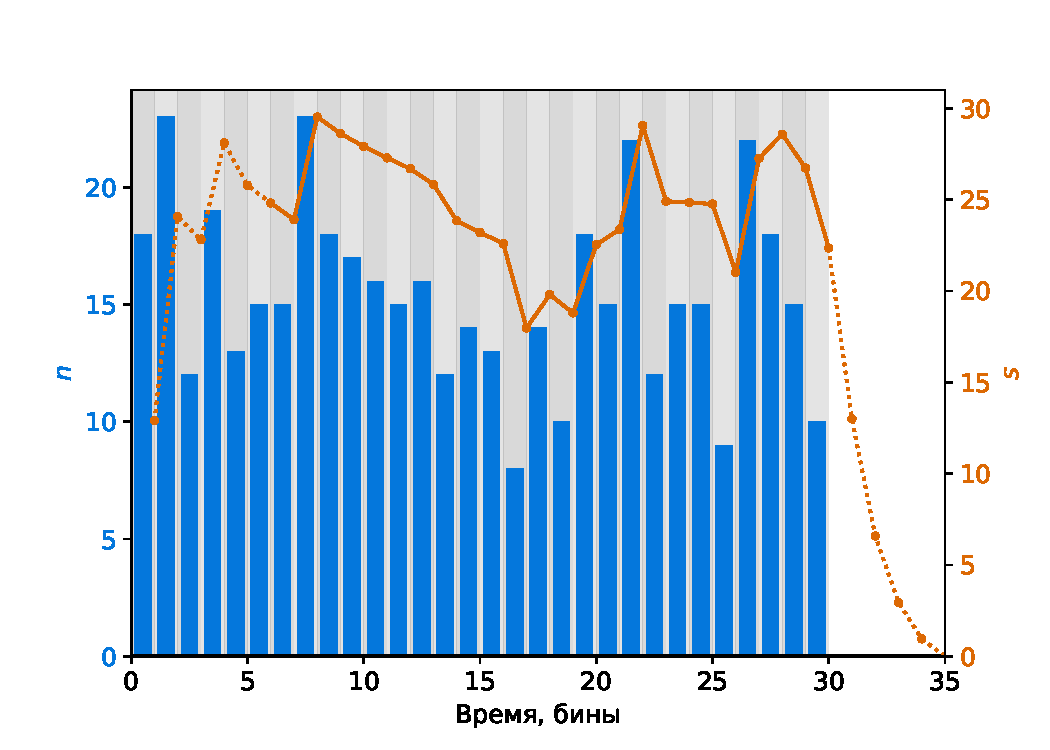
\includegraphics[width=\columnwidth]{problem-setup-example}
		\caption{Пример входных и выходных данных для задачи байесовской деконволюции. РИХ определена выражениями (\ref{eq:example-problem-rir}); пунктиром показаны участки, исключаемые из рассмотрения для устранения эффекта окна.}
		\label{pic:problem-setup}
	\end{figure}
	
	Иллюстрация $\vec{n}$ и $\vec{s}$ для этой демонстрационной задачи приведена на рис. \ref{pic:problem-setup}.
	
	\subsection{Эффект окна} \label{sec:edge-effects}
	
	В реальном эксперименте входные фотоны не ограничены интервалом $[0; N]$, но приходят постоянно. Модифицируем постановку задачи так, чтобы устранить эффект окна, то есть влияние  -- плавный рост сигнала в начале и затухание в конце.
	
	Для этого достаточно исключить из всего дальнейшего рассмотрения эти участки сигнала. Так, в реальной ситуации фотоны продолжают приходить после $t=N$, и вносят соответствующий вклад в отсчёты начиная с $N-1$. Фотоны, приходившие до $t=0$, вносят вклад в отсчёты до $L$.
	
	Поэтому для восстановления значений $n_i$, $i = 1, \ldots, N$ мы будем использовать только отсчёты $S_j$ при $j = L+1, \ldots, N$. Этот участок изображён на рис. \ref{pic:problem-setup} сплошной линией, участки по краям, исключаемые из рассмотрения -- пунктиром.
	
	
	\section{Постановка задачи}
	
	Поставим задачу статистической деконволюции следующим образом, используя байесовскую терминологию (поэтому будем также называть эту процедуру байесовской деконволюцией):
	
	\begin{quote}
		Пусть дана рандомизированная импульсная характеристика системы $\tilde{h}(t)$ и значения $s_j, \; j = 1, \ldots, N + L$. Найти апостериорные функции плотности вероятности для значений $n_i$, $i = 1, \ldots, N$.
	\end{quote}
	
	Заметим, что, в отличие от обычной деконволюции, мы не ставим задачу оценить исходный сигнал сам по себе, представляющий собой сумму $\delta$-функций, но только его несколько обобщённую характеристику.

	\section{Решение}

	\subsection{Выходной сигнал как реализация случайного процесса}
	
	Ясно, что в силу случайного характера отклика системы, а также аггрегирования фотонов в бины, значения отсчётов $\{ s_j \}$ являются реализациями некоторых случайных величин. Обозначим сами эти случайные величины как $\{ S_j \}$.

	Запишем $S_j$ как сумму вкладов от фотонов разных бинов
	
	\begin{equation}
		S_j = \sum_{l=0}^{L} C(n_{j-l}, l)
		\label{eq:S-definition-as-random-variable}
	\end{equation}

	Здесь $C(n, l)$ -- случайная величина, описывающая вклад в сигнал на $j$-том временном отсчёте от $n$ фотонов в бине $j - l$, иначе говоря, вклад с \textit{задержкой} $l$ бинов. Из выбранной схемы индексации бинов и условий каузальности и ограниченности во времени РИХ легко видеть, что $l \in \left[0, L\right]$, поскольку вклад от фотонов более ранних бинов равен нулю.
	
	Охарактеризуем распределение $C(n, l)$. Проще всего сделать это через Монте-Карло-сэмплирование распределения этой величины. Получим сначала с произвольной точностью эмпирическую функцию плотности распределения для $C(1, l)$. Для этого сгенерируем значения $t_k \sim t_{inbin};$ и функции $h_k(t) \sim \tilde{h}(t)$ для $k = 1 \ldots N_{sample}$. Выборка для $C(1, l)$ тогда будет состоять из значений $h_k(l + 1 - t_k)$. Выборка для $C(n, l)$ легко получить, проделав описанную процедуру $n$ раз и сложив все $n$ реализаций $N_{sample}$-мерных векторов выборок.

	\subsection{Грубая оценка}
	\label{sec:rough-estimation}
	
	Перед тем, как решать задачу деконволюции в статистическом смысле, сделаем грубую оценку $\vec{n}$, основанную только на соотношениях между математическими ожиданиями случайных величин. Для этого применим операцию вычисления математического ожидания к обеим частям равенства (\ref{eq:S-definition-as-random-variable}).
	
	Фотоны независимы друг от друга в пределах одного бина, из чего следует $ \mathbb{E} \; C(n, l) = n \; \mathbb{E} \, C(1, l)$. Нетрудно заранее вычислить для данной РИХ выборки значений $C(1, l)$ для $l = 0 \ldots L$. Тогда получим, обозначая $c_l \equiv \mathbb{E} \; C(1, l)$,
	
	\begin{equation}
		\bar{S}_j = \mathbb{E} \; S_j = \sum_{l=0}^{L} \mathbb{E} \; C(n_{j-l}, l) = \sum_{l=0}^{L} n_{j-l} \; \mathbb{E} \; C(1, l) = \sum_{l=0}^{L} n_{j-l} c_l
	\end{equation}

	Суммирование можно записать в матричном виде для $j = 1, \ldots, N + L$:
	
	\begin{equation}
		\begin{pmatrix} 
			c_0   &  0   &  0   &\dotsm&  0     \\
			c_1   & c_0  &  0   &\dotsm&  0     \\
			c_2   & c_1  & c_0  &      & \vdots \\
			c_3   & c_2  & c_1  &\ddots&  0     \\
     	    \vdots& c_3  & c_2  &\ddots&  c_0   \\
			c_L   &\vdots& c_3  &\ddots&  c_1   \\
			0     & c_L  &\vdots&\ddots&  c_2   \\
			\vdots&      & c_L  &      &  c_3   \\
			0     &\dotsm&  0   &\ddots& \vdots \\
			0     &\dotsm& 0    &   0  &  c_L   \\
		\end{pmatrix}
		\begin{pmatrix} 
			n_1 \\ n_2 \\ n_3 \\ \vdots \\ n_N
		\end{pmatrix}
		=
		\begin{pmatrix} 
			\bar{S}_1 \\ \bar{S}_2 \\
			\vdots \\
			\bar{S}_N \\ \bar{S}_{N+1} \\
			\vdots \\
			\bar{S}_{N+L}
		\end{pmatrix}
		\label{eq:mean-vector-calculation}
	\end{equation}

	Для исключения граничных эффектов, и тем самым перехода к случаю непрерывного потока фотонов достаточно, как указано в разделе \ref{sec:edge-effects}, ограничиться рассмотрением строк $j = L+1, \ldots, N$, то есть убрать первые и последние $L$ уравнений системы.

	Эта возможно несовместная система линейных уравнений, допускает решение в смысле наименьших квадратов с помощью псевдообратной матрицы Мура-Пенроуза \cite{Penrose1956}. Псевдообратная матрица $C^+$ для $C$ определяется следующими условиями: (1) $C C^+ C = C$, (2) $C^+ C C^+ = C^+$, (3) $C C^+$ и $C^+ C$ -- эрмитовы матрицы. Псевдообратная матрица всегда существует, и для системы $C\vec{n} = \vec{S}$ вектор $C^+ \vec{S}$ даёт искомое МНК-решение системы. Приближённый численный расчёт такой матрицы можно провести, например, с помощью функции \verb|pinv| модуля \verb|numpy.linalg| в Python \cite{Harris2020}.

	\begin{figure}
		\centering
		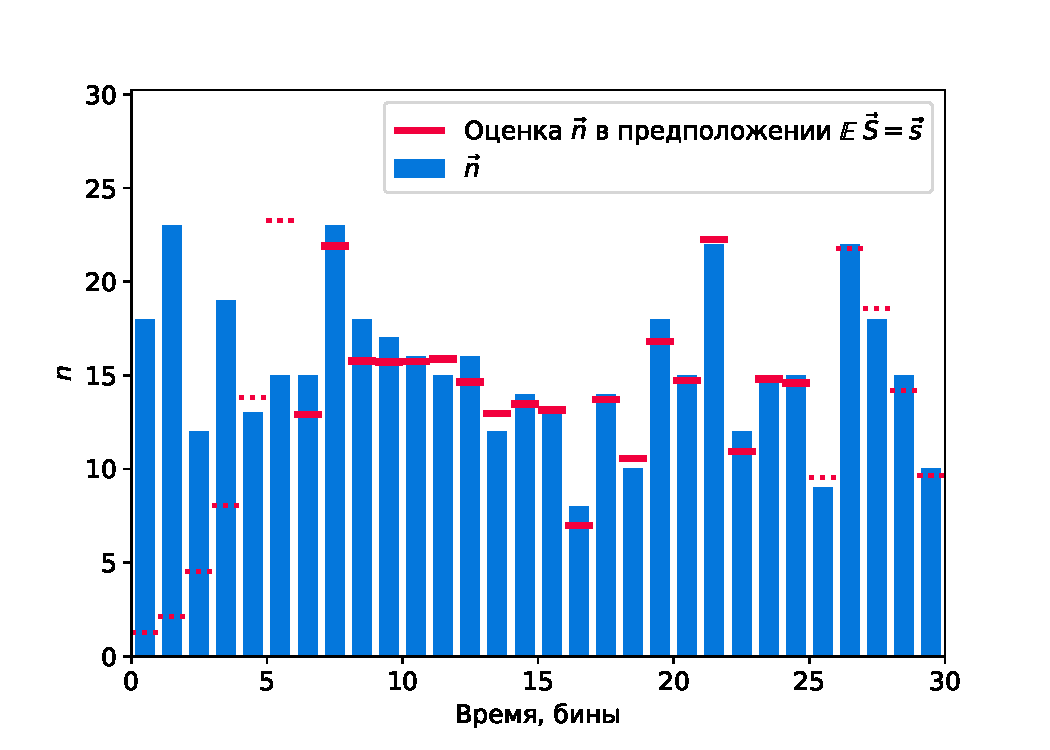
\includegraphics[width=\columnwidth]{mean-estimation}
		\caption{Оценка $\vec{n}$ в предположении, что выходной сигнал $\vec{s}$ равен своему математическому ожиданию. Пунктиром показана область, где оценка искажена эффектом ограниченности выборки во времени.}
		\label{pic:mean-estimation}
	\end{figure}
	
	Однако для решения системы необходимо знать $\mathbb{E} \, S_j$, в то время как в эксперименте мы имеем всего лишь единственную реализацию этой случайной величины $s_j$. Для грубой оценки остаётся положить $\mathbb{E} \; S_j \approxeq s_j$. Результат описанной процедуры приведён на рис. \ref{pic:mean-estimation} фиолетовым, пунктиром отмечена область, в которой оценка искажена эффектом окна.
	
	\begin{figure}
		\centering
		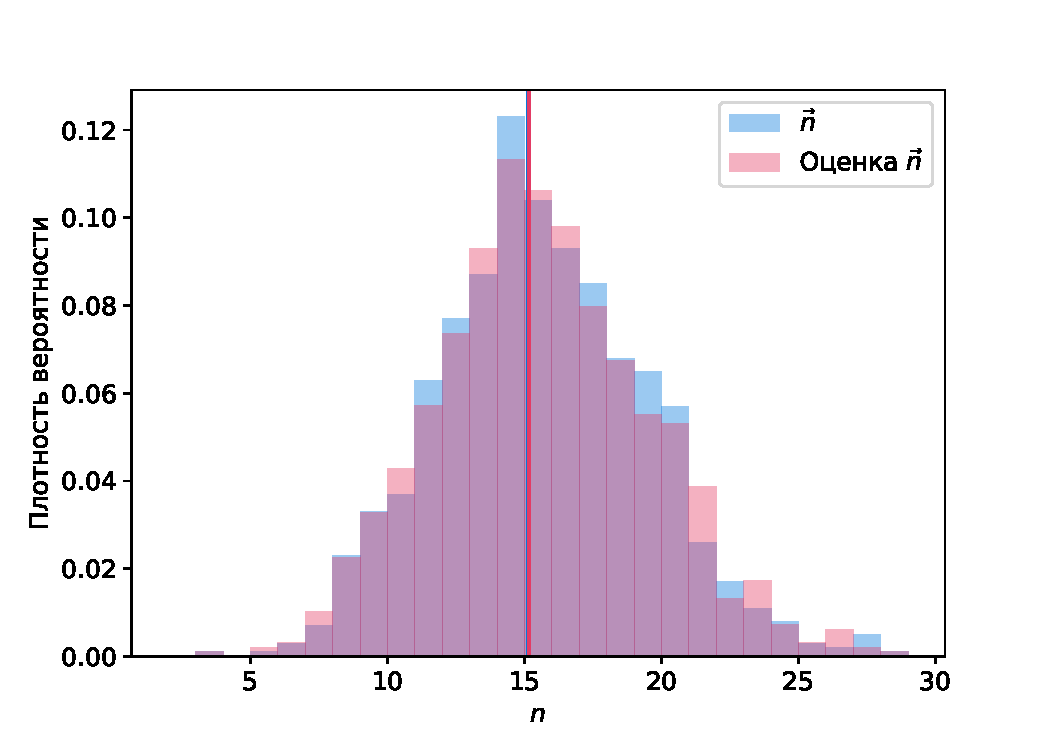
\includegraphics[width=\columnwidth]{mean-estimation-assessment}
		\caption{Распределения истинных и грубо восстановленных значений $\vec{n}$ для 1000 значений. Истинные значения выбраны из пуассоновского распределения с $\lambda = 15$, аналогично рис. \ref{pic:problem-setup} и \ref{pic:mean-estimation}.}
		\label{pic:mean-estimation-assessment}
	\end{figure}
	
	Строгое исследование свойств такой <<one-shot>> оценки $\vec{n}$ находится за рамками данной работы. Однако для простой численной проверки можно провести описанную процедуру для большего числа входных бинов и сравнить распределения истинных и оцененных значений $\vec{n}$. На рис. \ref{pic:mean-estimation-assessment} приведено такое сравнение для 1000 бинов. Видно, что распределения практически совпадают, а значит отсутствует по крайней мере систематическая ошибка. В дальнейшем эта оценка будет играть роль первого приближения, или стартовой точки, на основе которой уже полными статистическим методом можно найти полное решение.
	
	\subsection{Решение задачи байесовской деконволюции}
	\label{sec:bayesian-deconvolution-solution}
	
	Теперь перейдём к решению полноценной статистической задачи, используя метод, описанный в предыдущем разделе, как первое приближение.
	
	Запишем сначала теорему Байеса в общем виде, учитывая, что наблюдаемыми значениями является сигнал $\vec{s}$, а неизвестными параметрами, которые задают распределение наблюдаемых -- $\vec{n}$:
	
	\begin{equation}
		P(\vec{n} | \vec{s}) = \frac{P(\vec{s} | \vec{n}) \, P(\vec{n})}{P(\vec{s})}
	\end{equation}

	Поясним вероятности, входящие в выражение: 
	
	\begin{enumerate}
		\item $P(\vec{n} | \vec{s})$ -- искомое \textit{апостериорное} распределение, описывающее (в байесовском определении вероятности) наши знания о $\vec{n}$ после проведения измерений
		\item $P(\vec{s} | \vec{n}) \equiv \mathcal{L}(\vec{s}, \vec{n})$ -- функция правдоподобия, описывающая, насколько вероятна регистрация определённых значений $\vec{s}$ при заданных параметрах $\vec{n}$
		\item $P(\vec{n}) \equiv \pi(\vec{n})$ -- \textit{априорное} распределение $\vec{n}$, не требующее знаний о конкретном выходном сигнале
		\item $P(\vec{s})$ -- полная вероятность регистрации данного сигнала при всех возможных значениях $\vec{n}$. Она также называемая маргинальной вероятностью или нормировочным множителем, по определению $P(\vec{s}) = \int_{\infty} P(\vec{s} | \vec{n}) \, P(\vec{n}) d\vec{n}$. Эту величину можно использовать для сравнения моделей, например, если бы мы имели в распоряжении альтернативную модель генерации значений $\vec{s}$ и хотели бы понять, какая из двух лучше описывает данные. Однако для поставленной задачи нет нужды ни вычислять, ни даже учитывать этот множитель.
	\end{enumerate}

	Учитывая введённые обозначения, запишем

	\begin{equation}
		\label{eq:bayes-theorem-adapted}
		P(\vec{n} | \vec{s}) \propto \mathcal{L}(\vec{s}, \vec{n}) \, \pi(\vec{n})
	\end{equation}

	\subsubsection{Выбор априорного распределения}
	
	В качестве априорного распределения будем использовать неограниченное равномерное, или \textit{неинформативное} распределение. Методы байесовской статистики работают даже в ситуации, когда у нас нет вообще никакой информации о распределении $\vec{n}$ до начала измерений. Формально для этого нужно положить $\pi(\vec{n}) = Const \; \forall \vec{n}$. Такое распределение нельзя использовать напрямую, поскольку его невозможно отнормировать на $1$. Однако тогда в выражении \ref{eq:bayes-theorem-adapted} можно просто исключить $\pi(\vec{n})$ из правой части.

	\subsubsection{Полное вычисление функции правдоподобия методом Монте-Карло}
	
	\label{sec:naive-monte-carlo-likelihood}

	Функция правдоподобия $\mathcal{L}(\vec{s}, \vec{n})$ определяется как вероятность того, что данный сигнал $\vec{s}$ получился в результате преобразования системой входного сигнала $\vec{n}$.

	Опишем сначала Монте-Карло метод оценки правдоподобия, и затем введём упрощения, которые позволят эффективнее вычислять эту функцию, а также обоснуем корректность этих упрощений. Для этого при фиксированных $\vec{n}$ необходимо смоделировать выборку из большого числа реализаций случайной величины $\vec{S}$, а затем оценить плотность вероятности в точке $\vec{s}$ по этой выборке.
	
	Существует несколько методов для такой оценки, самый простой из которых -- многомерная гистограмма. Для этого пространство реализаций $\vec{S}$ нужно поделить на ячейки, подсчитать число элементов выборки, попавших в каждую ячейку, и поделить на общее число элементов выборки и на объём ячейки. Нетрудно видеть, что полученное число даст оценку плотности вероятности в произвольной точке -- а значит, искомую оценку функции правдоподобия.
	
	Однако оказывается, что для поставленной задачи метод прямого вычисления функции правдоподобия плохо годится из-за <<проклятия размерности>>. Размерность пространства, в котором нужно оценить эмпирическую функцию плотности вероятности, равна ширина окна, в котором рассматривается входной сигнал, в бинах. Соответственно, общее число $N$-мерных бинов составляет $g^{N}$, где $g$ -- мощность бинирования каждого отсчёта. В этой ситуации для надёжной оценки придётся генерировать выборку сравнимого объёма.
	
	Поэтому вместо прямого использования описанного метода аппроксимируем распределение $\vec{S}$ более вычислительно эффективной функцией.

	\subsubsection{Аппроксимация функции правдоподобия многомерным нормальным распределением}
	
	\label{sec:likelihood-as-multivar-normal}
	
	Проанализируем результат полной Монте-Карло симуляции, чтобы исследовать распределение $p(\vec{S} | \vec{n})$ и показать, что его в самом деле можно эффективно и с высокой точностью аппроксимировать многомерным нормальным распределением.
	
	\paragraph{Частные распределения}

	Из самых общих соображения ясно, что распределение $S_j \forall j$ будет более или менее близко к нормальному -- просто в силу того, что каждая из $S_j$ является суммой независимых (хотя и не всех одинаково распределённых) вкладов от фотонов в предыдущих бинах. Также сразу можно сказать, что \textit{чем меньше среднее число фотонов в бине, тем хуже будет аппроксимация нормальным распределением}. На рис. \ref{pic:s-j-norm-assess} приведены несколько распределений <<лучшего>>, <<медианного>> и <<худшего>> распределений $S_j$ для нескольких значений среднего числа фотонов в бине $\lambda_n \equiv \mathbb{E} \, n_i$. Из предварительного анализа и независимых соображений известно, что менее $5$ фотонов на бин -- весьма нечастая ситуация в экспериментальных данных -- но даже в этом случае видно, что самое существенное среднеквадратичное отклонение плотности распределения от гауссианы не превышет 10\%. Таким образом, \textit{частное распределение} каждой компоненты вектора $\vec{S}$ можно приблизить нормальным распределением с эффективной погрешностью в несколько процентов для практически значимых случаев.
	
	\begin{figure}
		\centering
		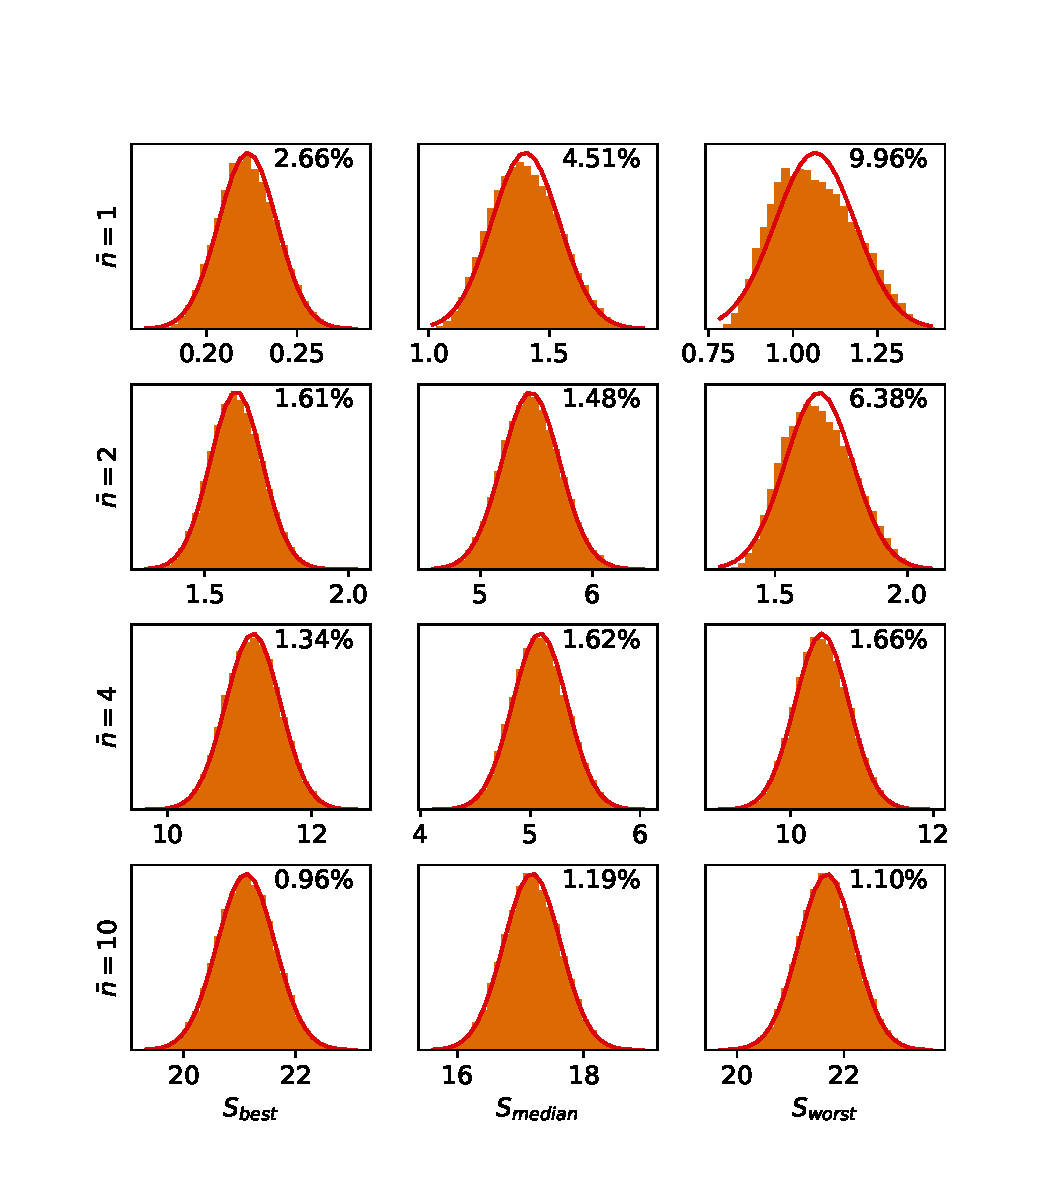
\includegraphics[width=\columnwidth]{S-j-normality-assessment.pdf}
		\caption{Оценка нормальности частных распределений компонент $\vec{S}$ для разных интенсивностей входного потока: от экстремально низких $1$ и $2$ до средней ожидаемой $10$. <<Лучший>>, <<медианный>> и <<худший>> бины определены эвристически по квадрату разницы выборочного среднего и медианы (чем больше эта величина, тем менее симметрично распределение). На каждом графике построена плотность нормального распределения с соответствующими $\mu$ и $\sigma$, а также приведено среднеквадратичное отклонение гистограммы от гауссианы в процентах относительно максимального значения.}
		\label{pic:s-j-norm-assess}
	\end{figure}

	\begin{figure}
		\centering
		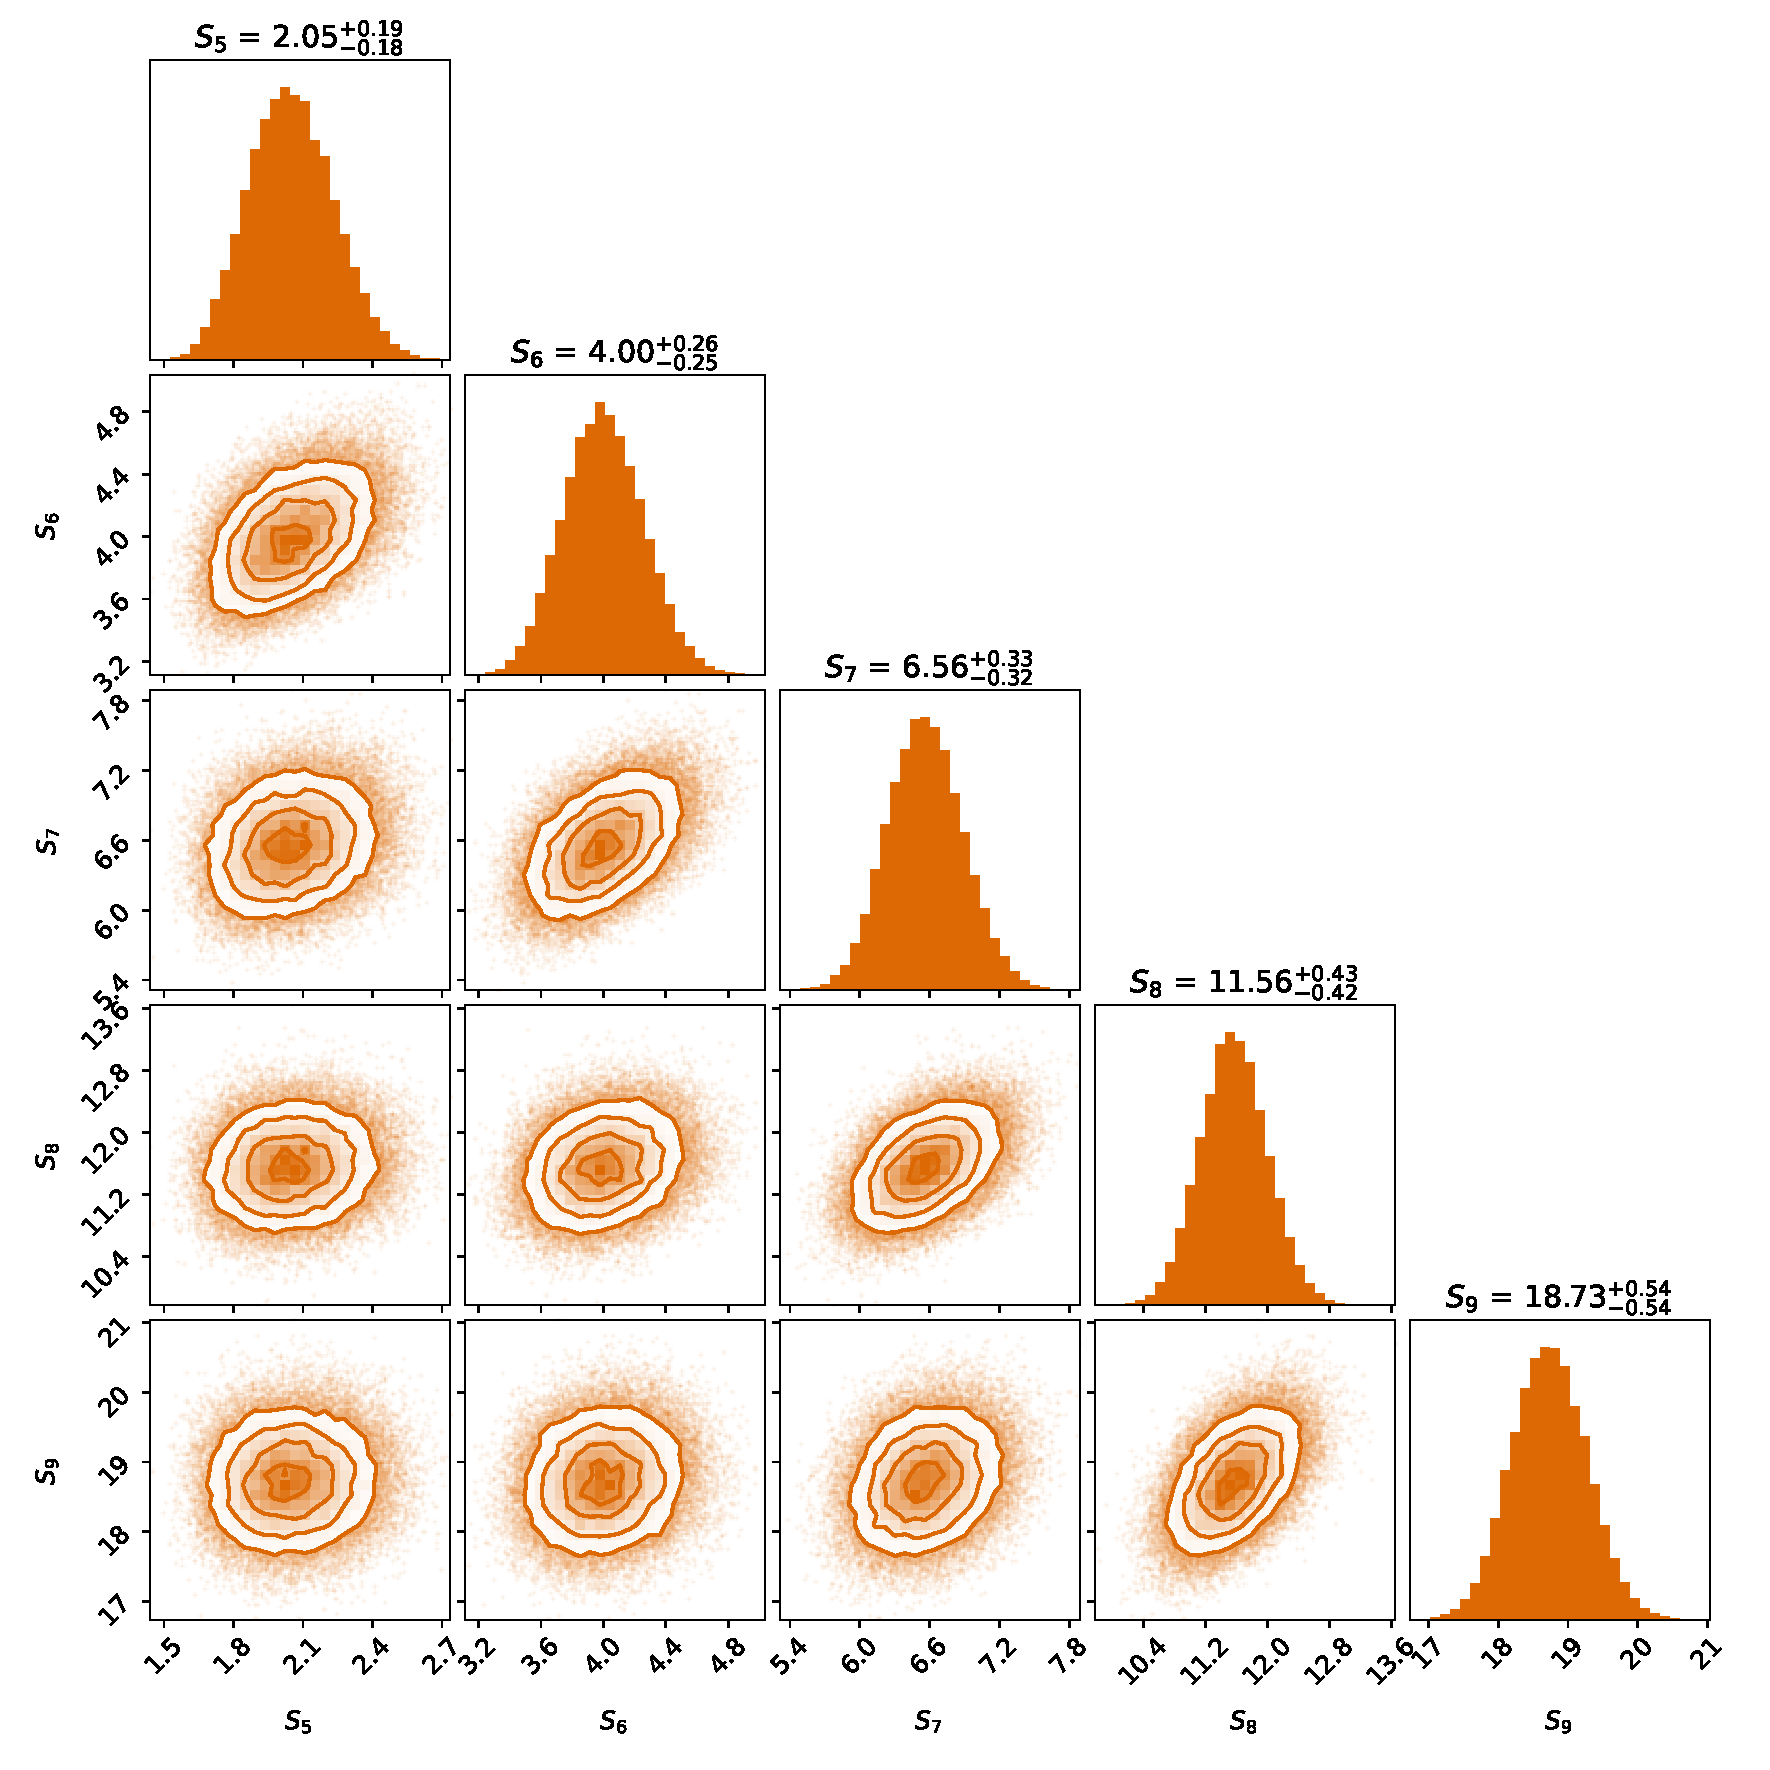
\includegraphics[width=1.2\columnwidth]{S-j-pairwise-normality-assessment.pdf}
		\caption{Оценка нормальности совместных двумерных распределений для пар компонент $\vec{S}$. График построен с помощью библиотеки corner \cite{ForemanMackey2016}.}
		\label{pic:s-j-pairwise-norm-assess}
	\end{figure}

	\paragraph{Полное $(N-L)$-мерное распределение}
	Провести аналогичную процедуру для полного $(N-L)$-мерного распределения -- непростая задачу, поэтому ограничимся здесь визуальным исследованием двухмерных распределений для пар $(S_j; S_k)$ для $k - j < L$ (из постановки задачи ясно, что на б\'{о}льших расстояниях элементы $\vec{S}$ независимы). На рис. \ref{pic:s-j-pairwise-norm-assess} представлены такие распределения. Видно, что двухмерные распределения представляют собой овалы симметричной формы, как и ожидается от многомерного нормального распределения.
	
	Таким образом, можно положить, что \textit{распределение вектора $\vec{S}$ при заданных $\vec{n}$ можно приблизить многомерным нормальным распределением}. Это приближение существенно упрощает вычисление функции правдоподобия $\mathcal{L}(\vec{n}) \equiv P(\vec{S} | \vec{n})$, которая и сводится к вычислению плотности вероятности условного распределения $\vec{S}$ в точке, заданной наблюдаемым сигналом. Этот метод оказывается гораздо более устойчивым и вычислительно эффективным, чем наивный метод Монте-Карло, описанный в разделе \ref{sec:naive-monte-carlo-likelihood}.

	Многомерное нормальное распределение в общем виде задаётся вектором математических ожиданий $\vec{\mu}$ и матрицой ковариаций $\Sigma$. Функция плотности вероятности $(N+L)$-мерного случайного вектора $\vec{S}$ тогда вычисляется как
	
	\begin{equation}
		\label{eq:multivariate-normal-density}
		p(\vec{S}) = \left( (2 \pi)^{N+L} \, \det \Sigma \right)^{-1/2} \exp \left( - \frac{1}{2} (\vec{S} - \vec{\mu})^T \Sigma^{-1} (\vec{S} - \vec{\mu}) \right)
	\end{equation}

	Вектор $\vec{\mu} \equiv \mathbb{E} \, \vec{S}$ как функция $\vec{n}$ вычисляется в соответствии с выражением (\ref{eq:mean-vector-calculation}). Вычислим, аналогично, произвольный элемент матрицы $\Sigma_{ij} \equiv \cov\left( S_i, S_j \right)$ при заданном $\vec{n}$. В силу симметричности матрицы ковариаций можно положить для определённости $i \le j$. Запишем выражение (\ref{eq:S-definition-as-random-variable}) для двух интересующих нас элементов $\vec{S}$:
	
	\begin{align}
		S_i &= \sum_{l=0}^{L} C(n_{i-l}, l)\\
		S_j &= \sum_{k=0}^{L} C(n_{j-k}, k)
	\end{align}

	Источник возможной ненулевой ковариации этих величин -- члены, описывающие вклады фотонов из одного бина, но на разных задержках, все прочие слагаемые независимы. Условие, описывающее такие попарно-скоррелированные члены, получается из равенства индексов $n$ в суммах: $i-l = j-k$. Вводя $\Delta \equiv j - i$, отсюда получаем $k = l + \Delta$. Отсюда сразу следует интуитивный вывод о том, что при $\Delta > L$ ковариация будет заведомо нулевой в силу конечности РИХ во времени.

	Используем следующее свойство ковариации: если $x$, $y$, $\epsilon$, $\eta$ -- случайные величины, из которых только $x$ и $y$ являются зависимыми, то $\cov(x + \epsilon, y + \eta) = \cov(x, y)$. Иначе говоря, заведомо независимые члены при вычислении ковариации можно просто опустить. Проделаем это в суммах выше, получив таким образом <<скореллированные части>> $\hat{S}_i$ и $\hat{S}_j$ такие, что $\cov ( S_i, S_j  ) = \cov ( \hat{S}_i, \hat{S}_j )$:
	
	\begin{align}
		\hat{S}_i &= \sum_{l=0}^{L-\Delta} C(n_{i-l}, l)\\
		\hat{S}_j &= \sum_{k=\Delta}^{L} C(n_{j-k}, k) = \left[k=l+\Delta\right] = \sum_{l=0}^{L-\Delta} C(n_{i-l}, l+\Delta)
	\end{align}

	Наконец, используем ещё одно свойство ковариации: если среди случайных величин $x_1$, $x_2$, $y_1$, $y_2$ независимы все пары, кроме $x_1$ и $y_1$, $x_2$ и $y_2$, то $\cov(x_1 + x_2, \, y_1 + y_2) = \cov(x_1, y_1) + \cov(x_2, y_2)$. Индуктивно обобщая на случай сумм с произвольным числом членов, и принимая во внимание, что фотоны в разных бинах независимы, получаем
	
	\begin{equation}
		\cov(S_i, S_j) = \cov(\hat{S}_i, \hat{S}_j) = \sum_{l=0}^{L - \Delta} \cov(C(n_{i-l}, l), C(n_{i-l}, l + \Delta))
	\end{equation}

	Наконец, принимая во внимание, что сама по себе величина $C(n, l)$ есть сумма $n$ независимых одинаково распределённых случайных величин, а между членами сумм $C(n, l)$ и $C(n, l + \Delta)$ есть только попарные корреляции в отношении 1 к 1, можно записать окончательную формулу для вычисления элемента матрицы ковариации:
	
	\begin{equation}
		\cov(S_i, S_{i + \Delta}) = \sum_{l=0}^{L - \Delta} n_{i-l} \; \cov\left(C(1, l), C(1, l + \Delta)\right)
	\end{equation}

	Из формулы видно, что автокорреляция сигнала описана полностью в терминах автокорреляции РИХ и чисел фотонов в соответствующих бинах, служащих весами для вклада разных участков РИХ.
	
	Для удобства вычислений можно записать это равенство в матричном виде для значений $\Delta \in \left[0; L\right]$. Для этого введём обозначение $\xi(l, \Delta) \equiv \cov\left(C(1, l), C(1, l + \Delta)\right)$ и с помощью него запишем:
	
	\begin{equation}
		\begin{pmatrix} 
			\xi(L, 0) & \xi(L-1, 0) & \xi(L-2, 0) & \dotsm & \xi(0, 0) \\
			     0    & \xi(L-1, 1) & \xi(L-2, 1) & \dotsm & \xi(0, 1) \\
				 0    &      0      & \xi(L-2, 2) & \dotsm & \xi(0, 2) \\
			   \vdots &   \vdots    &    \vdots   & \ddots &   \vdots  \\
			     0    &      0      &      0      & \dotsm & \xi(0, L)
		\end{pmatrix}
		\begin{pmatrix} 
			n_{i-L} \\ n_{i-(L-1)} \\ n_{i-(L-2)} \\ \vdots \\ n_{i}
		\end{pmatrix}
		=
		\begin{pmatrix} 
			\Sigma_{i, i} \\
			\Sigma_{i, i+1} \\ 
			\Sigma_{i, i+2} \\ 
			\vdots \\ 
			\Sigma_{i, i+L}
		\end{pmatrix}
		\label{eq:Xi-matrix-for-Sigma-calculation}
	\end{equation}

	Это достаточно неинтуитивное выражение позволяет, однако, единожды вычислить матрицу $\Xi$ и эффективно рассчитывать все элементы матрицы ковариаций $\Sigma$ при каждом заданном $\vec{n}$. Окончательное единое выражение для всей матрицы $\Sigma$ будет излишне громоздким, и при реальном вычислении не требуется -- достаточно просто составить её из векторов $\left( \Sigma_{i, i}, \dots, \Sigma_{i, i+L} \right)^T$, учитывая свойство симметрии $\Sigma_{i, j} = \Sigma_{j, i}$, а также доказанный факт $\Sigma_{i, j} = 0 \quad \forall j > i + L$
	
	После исключения областей влияния эффекта окна -- первых и последних $L$ элементов $\vec{S}$ -- нас будут интересовать только внутренняя часть матрицы $\Sigma$, то есть индексы $i, j \in [L + 1; N]$. Это удобно, так как для вычисления интересующей нас части $\Sigma$ не нужно рассматривать <<урезанную>> матрицу $\Xi$, что потребовалось бы, если бы мы не исключали границы.

	Таким образом, функция правдоподобия задаётся формулой (\ref{eq:multivariate-normal-density}), где вектор математических ожиданий и матрица ковариаций являются функциями $\vec{n}$ и вычисляются в соответствии с формулами (\ref{eq:mean-vector-calculation}) и (\ref{eq:Xi-matrix-for-Sigma-calculation}).
	
	\subsubsection{Сэмплирование апостериорного распределения}
	
	Имея функцию правдоподобия $\mathcal{L}$ и учитывая выбранные неинформативные априорные распределения, мы получаем функцию плотности апостериорной вероятности $P(\vec{n} | \vec{s}) \propto \mathcal{L}(\vec{n}, \vec{s})$, которую требуется исследовать.

	Требуется получить не только наиболее оптимальное значение $\vec{n}$, но и оценку неопределённости этой величины. Поэтому, например, простой метод максимального правдоподобия, в котором мы нашли бы максимум $\mathcal{L}$ в пространстве параметров, не подходит -- хотя существуют методы поиска доверительных интервалов. Мы будем использовать метод Монте-Карло с марковскими цепями (Markov Chain Monte Carlo), который хорошо применим к задачам большой размерности. Суть метода сводится к запуску марковского процесса случайного блуждания в пространстве параметров $\vec{n}$ с такой специально подобранной вероятностью перехода, зависящей от апостериорной вероятности, что в пределе это блуждание даст выборку из исследуемой функции плотности. Общей характеристикой этих методов является то, что они зависят только от отношения вероятностей в разных точках пространства параметров -- именно поэтому в выражении \ref{eq:bayes-theorem-adapted} и во всех последующих вычислениях мы не интересовались ни полной маргинальной вероятностью наблюдаемых данных, ни нормировкой априорного распределения.
	
	Подробный обзор и теоретическое исследование весьма широкой области MCMC-сэмплирования находятся за рамками данной работы, но могут быть найдены, например, в обзоре \cite{Sharma2017}.

	\paragraph{Афинно-инвариантное MCMC-сэмплирование}
	
	В данной работе будем использовать популярный алгоритм афинно-инвариантного сэмплирования, предложенный в 2010 году в работе \cite{Goodman2010}.
	
	В этом алгоритме используется не одна марковская цепь (англ. \textit{walker}), а целый ансамбль из нескольких сотен или даже тысяч цепей, и новый шаг генерируется для каждой цепи в зависимости от состояний остальных. Конкретный алгоритм генерации шага (или просто <<шаг>>, англ. \textit{move}) не фиксирован и может быть выбран в зависимости от конкретной задачи. Каждый из шагов обладает своими особенностями и по-своему влияет на предпочтительное количество цепей и необходимое количество итераций. Самый универсальный -- так называемый <<шаг-растяжка>> (англ. \textit{stretch move}), опишем его вкратце.
	
	Рассмотрим $i$-тую цепь, находящуюся в состоянии $X_i(t)$ (состояние цепи есть точка в пространстве параметров, иначе говоря, конкретное значение $\vec{n}$). Выберем случайным образом комплементарную цепь из ансамбля и обозначим её $X_j(t)$, $j \neq i$. Сгенерируем <<предложение>> (англ. \textit{proposal}) для данной цепи:
	\begin{equation}
		\label{eq:gw2010-stretch-move}
		Y = X_j(t) + Z \; (X_i(t) - X_j(t))
	\end{equation}

	Предложенное новое положение $i$-той цепи находится на прямой, соединяющей её с другой цепью на данном шаге. Масштабный множитель $Z$ -- случайная величина, на которую накладывается важное теоретическое ограничение: для существования стационарного распределения марковской цепи достаточно обеспечить детальное равновесие, то есть равенство вероятностей перехода $X_i \rightarrow Y$ и $Y \rightarrow X_i$. Для этого достаточно потребовать, чтобы функция плотности вероятности величины $Z$ должна удовлетворять свойству симметрии $g(1 / z) = z \, g(z)$. В качестве конкретного вида этой функции авторы предлагают 
	
	\begin{equation}
		g(z) \propto \begin{cases}
			\frac{1}{\sqrt{z}}& \text{при } z \in \left[\frac{1}{a}, a\right], \\
			0& \text{в остальных случаях }
		\end{cases}
	\end{equation}

	Наконец, после генерации предложения для нового положения $i$-той цепи (не важно, описанным шагом-растяжкой или любым другим алгоритмом) требуется принять или отвергнуть предложенное значение $Y$. Вероятность того или иного исхода получается из условия \textit{частичного ресэмплинга}, которое гласит: чтобы переход ансамбля цепей в новое состояние не менял совместного распределения всего ансамбля (которое полагается равным целевому сэмплируемому распределению), достаточно, чтобы переход одной цепи не менял условную плотность вероятности для данной цепи при фиксированных всех остальных. В конце концов, это сложное условие сводится к обычному детальному равновесию, но записанному для всего ансамбля цепей. Вероятность принять предложение $Y$, обеспечивающая детальное равновесие, задаётся величиной
	
	\begin{equation}
		P(X_i(t + 1) = Y) = min \left\{ 1, \; Z^{N - 1} \frac{p(Y)}{p(X_i(t))} \right\}
	\end{equation}

	Упрощённо можно сказать, что цепи ансамбля будут с большей вероятностью переходить в области большего значения сэмплируемой функции (то есть исследуемой плотности апостериорной распределения), но при этом также чаще оставаться вблизи <<соседей>> по ансамблю.

	\paragraph{Имплементация MCMC-сэмплирования в пакете emcee}
	
	\label{sec:mcmc-implementation-details}

	Эффективная и устойчивая реализация алгоритма MCMC-сэмплирования представляет собой непростую задачу. В приложении \textbf{TBD} приведена авторская реализация процедуры в \verb|MATLAB|, однако в дальнейшем будет использоваться популярная имплементация описанного алгоритма в пакете \verb|emcee| на языке \verb|Python| \cite{ForemanMackey2016}.

	Пакет предоставляет возможность не только провести сэмплирование, но и оценить корректность результата. Строгое математическое доказательство позволяет установить только \textit{асимптотическую} сходимость ансамбля цепей к целевому распределению. При этом реальная длина цепей конечна, и степень сходимости требует отдельной оценки -- иначе говоря, количество шагов должно быть \textit{достаточно большим} для использования результата.
	
	Но даже если ансамбль сошёлся с хорошей точностью, из него ещё требуется получить выборку независимых реализаций случайной величины. Состояние ансамбля на конкретном (например, последнем) шаге даёт ряд значений, однако число цепей в ансамбле чаще всего меньше, чем желаемое количество элементов выборки -- а значит, приходится брать значения на нескольких шагах. Шаги каждой цепи принципиально зависимы, но корреляция падает с расстоянием -- следовательно, для получения выборки нужно выбирать \textit{достаточно редкие} состояния ансамбля цепей.

	На практике эти две проблемы выражаются в необходимости выбрать время <<разгона>> (англ. \textit{burn-in}) и <<прореживание>> (англ. \textit{thinning}) цепей. Информированный выбор обоих параметров можно провести с помощью оценки \textit{интегрированного времени автокорреляции} $\tau$ \cite{Sokal1997}. Интегрированное время автокорреляции даёт оценку числа шагов, на котором корреляция значений цепи падает в $e$ раз. Соответственно, период разгона можно взять равным нескольким $\tau$, и прореживать значения не реже чем каждые $\tau$ шагов. Пакет \verb|emcee| предоставляет готовые средства для оценки величины $\tau$ \footfullcite{emceeAutocorrTutorial}.
	
	\begin{figure}
		\centering
		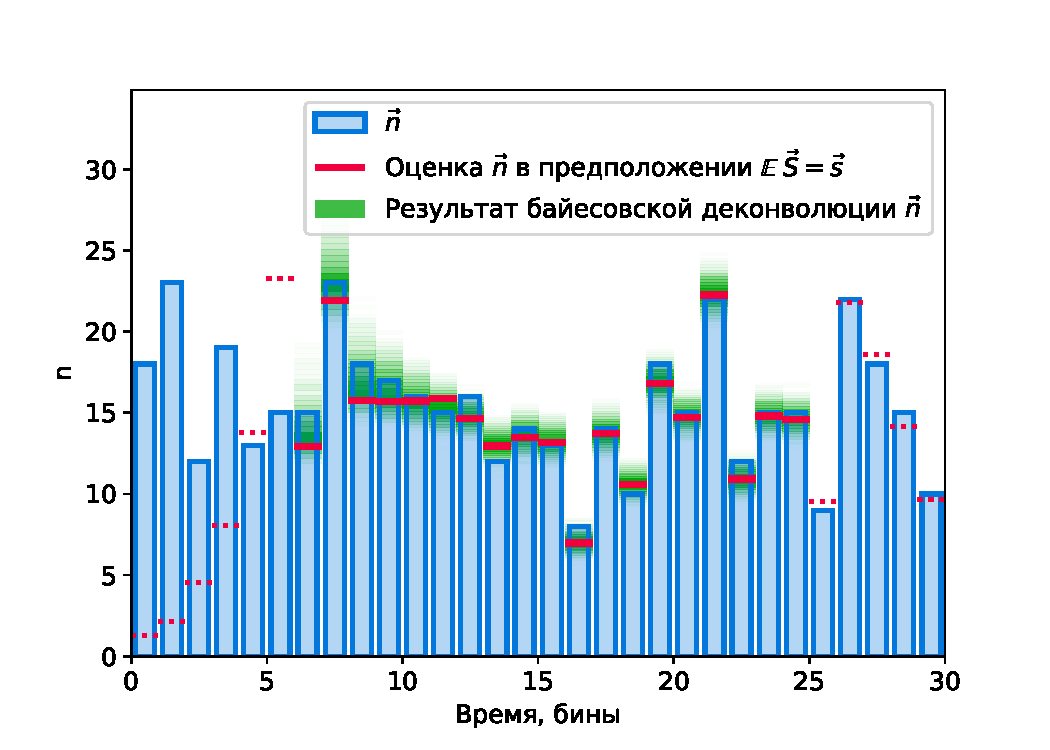
\includegraphics[width=\columnwidth]{bayesian-estimation-result}
		\caption{Результат решения задачи байесовской деконволюции. Зелёным показаны \textit{маргинальные апостериорные распределения}, то есть однопараметрические проекции апостериорного распределения как функции $n_i$ для области $i$, не подверженной влиянию эффекта окна. Следует заметить, что на самом деле многомерное апостериорное распределение не обязательно факторизуемо, поэтому для дальнейшего анализа нельзя рассматривать маргинальные распределения по отдельности -- они приведены только для иллюстрации результата.}
		\label{pic:bayesian-estimation}
	\end{figure}

	Более подробное описание конфигурации сэмплера и контроля качества сэмплирования приведено в разделе \textbf{TBD}, так как оно зависит от конкретной используемой РИХ.

	Помимо метапараметров (количество цепей, параметр $a$ для <<шага-растяжки>> или соответствующих параметров для других шагов) важной является инициализация сэмплера. Несмотря на теоретически предсказываемое <<забывания>> состояния цепей в течении нескольких $\tau$, в большинстве практических задач начальное положение цепей желательно задавать разумным образом. Здесь пригодится результат раздела \ref{sec:rough-estimation} -- простым и быстрым способом можно получить $\vec{n}_{rough}$ -- грубую оценку $\vec{n}$. Следуя практической рекомендации из статьи \cite{ForemanMackey2016}, инициализируем $N_{walker}$ цепей значениями, близкими к этой оценке, но дополнительно разбросанными в соответствии с нормальным распределением числа фотонов в каждом бине. Стандартное отклонение этого начального разброса должно быть заметно меньше разброса самих данных\footnote{\textquote[\cite{ForemanMackey2016}]{Another general approach is to start the walkers in a very tight N-dimensional ball in parameter space around one point that is expected to be close to the maximum probability point.}}, например $\hat{\sigma}_{rough} / 10$, где $\hat{\sigma}_{rough}$ -- выборочное стандартное отклонение, расчитанное по элементам $\vec{n}_{rough}$.
	
	Результат таким образом проведённого сэмплирования для демонстрационной задачи приведён на \ref{pic:bayesian-estimation}.



	\section{Деконволюция экспериментальных данных}
	
	Общий метод байесовской деконволюции, изложенный в предыдущем разделе, теперь применим к экспериментальным данным.
	
	В этом разделе будем рассматривать преобразование фотоэлектронов, испущенных фотокатодом ФЭУ под воздействием собранных фотонов, в импульс анодного тока, стекающего с его анодной RC-цепочки. На этом этапе преобразований сигнала определяется и временные характеристики (форма размытия импульса во времени зависит от параметров анодной цепи и собственной формы сигнала ФЭУ), и его амплитуда, причём значение последней носит случайный характер для каждого фотона, однако среднее её значение измеряется в процессе калибровки детектора. При этом, как описано в работе \cite{Sphere2015}, система <<ФЭУ + анодная схема + АЦП>> является линейной с высокой точностью, и небольшая коррекция нелинейности применяется к данным для компенсации тех небольших искажений, что всё же проявляются.

	Детальное описание схем подключения и питания ФЭУ, схему преобразования и усиления сигнала, а также характеристики использованных аналого-цифровых преобразователей можно найти в работе \cite{SphereDetector2020}.
	
	\subsection{Экспериментальная рандомизированная импульсная характеристика}

	Определим случайную функцию $\tilde{h}(t)$, которую будем использовать в качестве рандомизированной импульсной характеристики системы. Сначала факторизуем её следующим образом
	
	\begin{equation}
		\label{eq:experimental-rir}
		\tilde{h}(t) = C \, \tilde{C}_{PMT} \, h_I(t)
	\end{equation}

	Здесь
	
	\begin{enumerate}
		\item $h_I(t)$ -- функция времени, описывающая \textit{форму} импульсной характеристики, то есть безразмерная и нормированная таким образом, что её интеграл равен 1. Эта функция известна из лабораторного измерения, оно же показывает, что форму можно считать одинаковой для всех 109 каналов мозаики. В этой функции мы феноменологически учитываем все физические процессы, искажающие сигнал во времени: фильтрацию импульса анодной RC-цепочкой, влияние длинной линии, по которой сигнал передаётся с мозаики ФЭУ к бортовому компьютеру, а также любые другие частотно-зависимые характеристики операционных усилителей или АЦП. График $h_I(t)$ изображён на верхней панели рис. \ref{pic:experimental-rir-params}.
		\item $\tilde{C}_{PMT}$ -- случайная величина, описывающая неопределённость коэффициента усиления ФЭУ. Лавинообразный процесс генерации вторичных электронов сильно зависит от случайных процессов, проходящих в области первого динода, и в зависимости от них коэффициент усиления также оказывается случайной величиной -- это и есть источник <<рандомизированности>> импульсной характеристики. $\tilde{C}_{PMT}$ безразмерна и масштабирована так, чтобы $\mathbb{E} \tilde{C}_{PMT} = 1$, плотность и функция распределения показана на нижней панели рис. \ref{pic:experimental-rir-params}. \textbf{Как получена -- описать процедуру общими словами, сослаться на приложение или private communication}
		\item $C$ -- коэффициент калибровки данного канала; размерность -- миллиамперы на фотоэлектрон. Процесс калибровки детектора СФЕРА-2 подробно описан в работе \cite{SphereCalibration2016}. Единственный размерный коэффициент, определяющий математическое ожидание интеграла от рандомизированной импульсной характеристики, то есть задающий усреднённую масштабную связь между $\vec{n}$ и $\vec{S}$.
	\end{enumerate}

	\begin{figure}
		\centering
		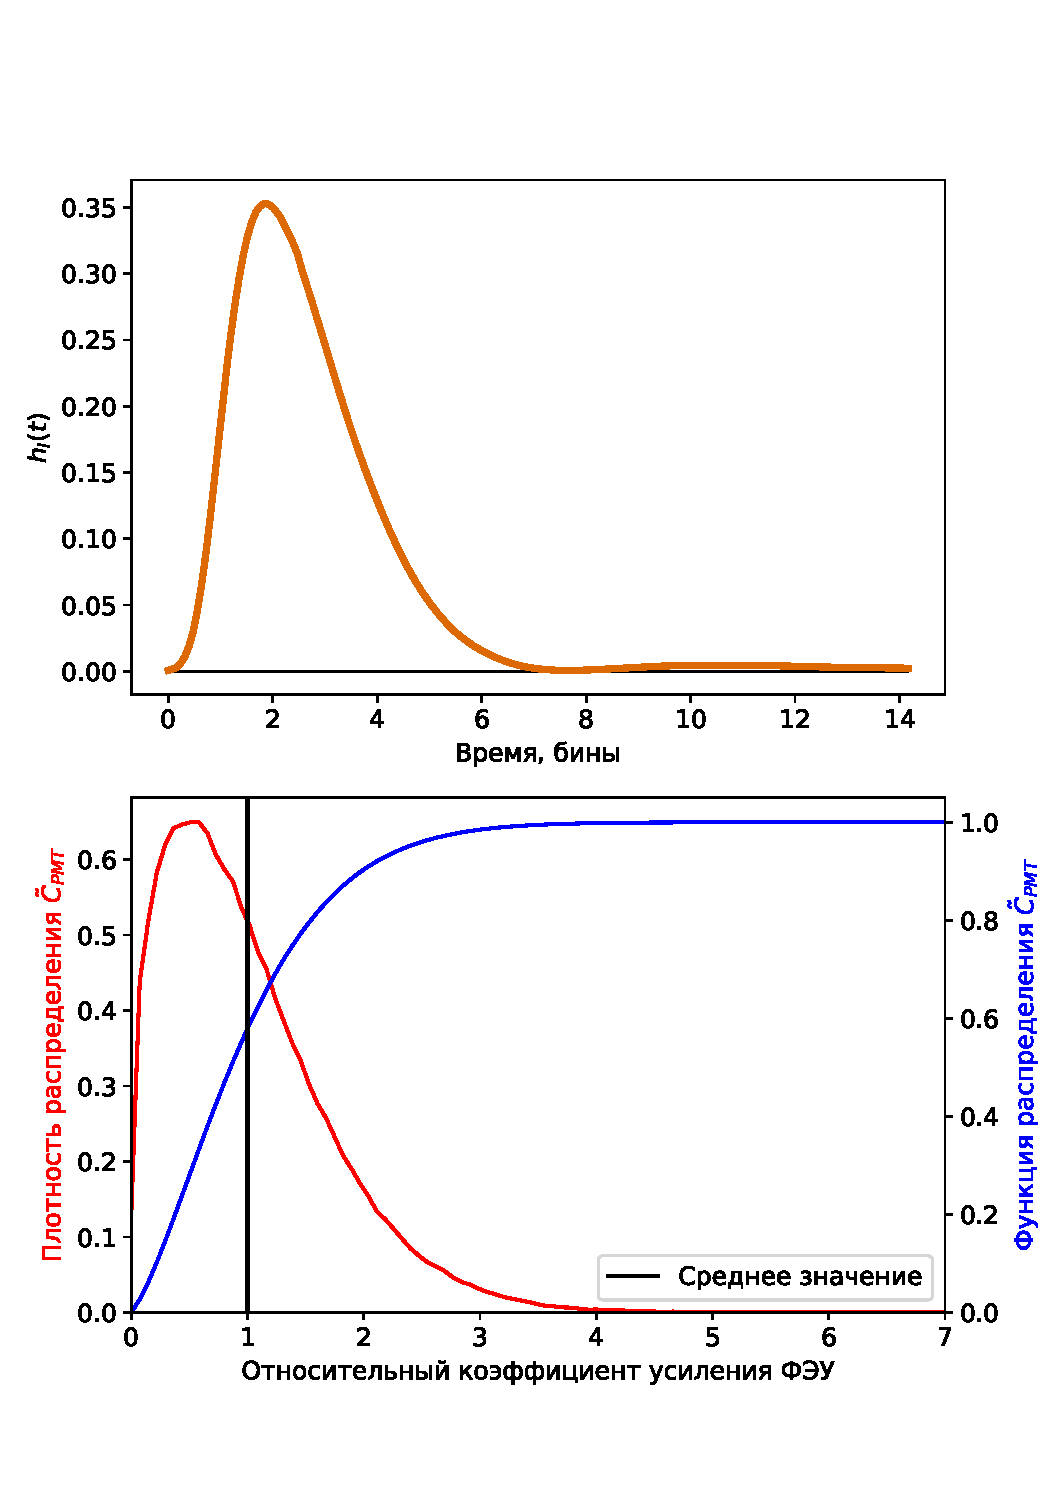
\includegraphics[width=\columnwidth]{experimental-ir-params}
		\caption{Компоненты экспериментальной рандомизированной импульсной характеристики. Функция $h_I(t)$ (верхняя панель) описывает форму импульса во времени, а случайная величина $\tilde{C}_{PMT}$ (функции распределения и плотности вероятности на нижней панели) -- неопределённость коэффициента усиления ФЭУ.}
		\label{pic:experimental-rir-params}
	\end{figure}

	Постоянный коэффициент калибровки $C$ не влияет на статистические свойства системы, и пока можно считать равным единице, его роль будет описана в разделе \textbf{TBD}.

	Получив РИХ, можно смоделировать отклик установки на определённый входной $\vec{n}$ и провести деконволюцию, чтобы оценить корректность работы метода, аналогично тому, как это было проделано с <<игрушечной>> РИХ (\ref{eq:example-problem-rir}). На рис. \ref{pic:bayesian-deconvolution-with-experimantal-rir} приведён результат такой процедуры. По сравнению с решением <<игрушечной>> задачи, приведённым на рис. \ref{pic:bayesian-estimation}, очевидна худшая точность деконволюции, что вполне объяснимо -- в первом случае РИХ быстро спадала во времени, была ограничена всего $L_1=10$ отсчётами, а её амплитуда варьировалась от $0.75$ до $1$; реальная РИХ, напротив, имеет широкий основной пик (около $5$ отсчётов) и длинный хвост, а её амплитуда варьируется в пределах от $0$ до $2$-$3$  относительно среднего значения. Однако в этом и состоит главное достоинство статистической деконволюции -- неполнота информации не ведёт к некорректности метода (что, вероятнее всего, случилось бы в случае с обыкновенной, детерминистичной деконволюцией, например, основанной на вычислении частного от фурье-образов), но предсказуемым образом отражается в результатах.
	
	\begin{figure}
		\centering
		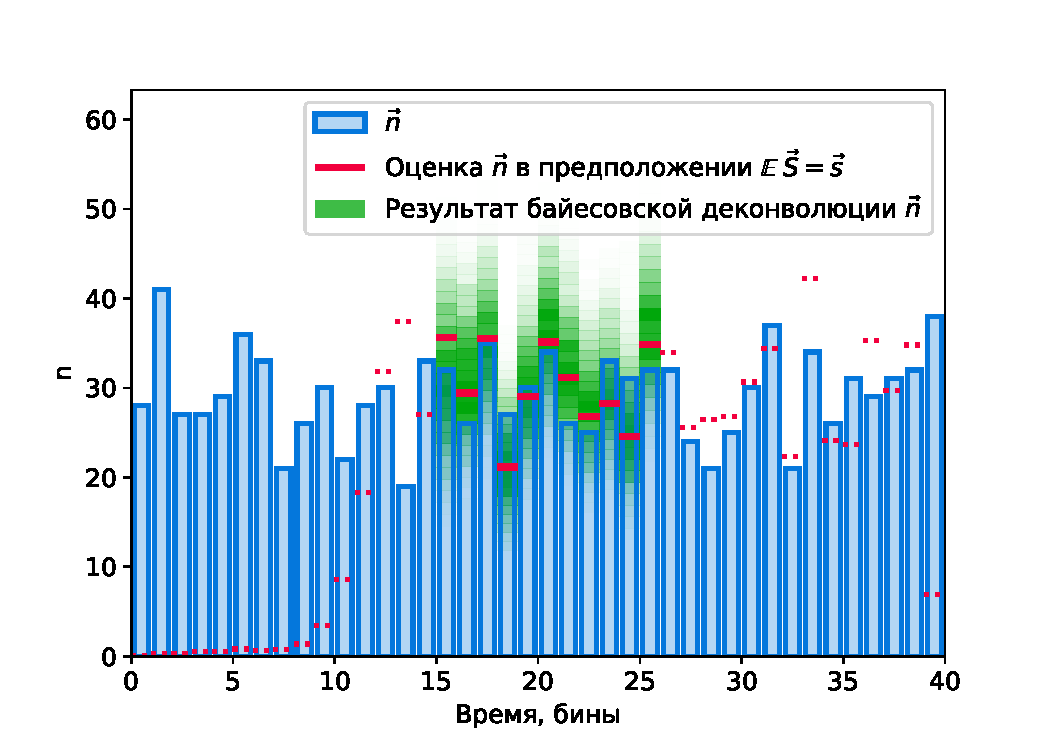
\includegraphics[width=\columnwidth]{bayesian-deconvolution-with-experimantal-rir}
		\caption{Решение задачи байесовской деконволюции для РИХ, определённой выражением (\ref{eq:experimental-rir}). Синие столбцы -- истинный входной сигнал $\vec{n}$, розовые полосы -- первичная грубая оценка, зелёным изображены маргинальные апостериорные распределения в центральных бинах (см. описание рис. \ref{pic:bayesian-estimation}).}
		\label{pic:bayesian-deconvolution-with-experimantal-rir}
	\end{figure}

	\subsection{Модификация процедуры для применения к реальным данным}
	
	Перед тем как, наконец, перейти от исследования метода к деконволюции реальных данных, необходимо внести две небольшие модификации в описанную процедуру.
	
	\subsubsection{Учёт неопределённости экспериментального сигнала}
	
	Функция правдоподобия, введённая в разделе \ref{sec:bayesian-deconvolution-solution}, и её аппроксимация, описанная в подразделе \ref{sec:likelihood-as-multivar-normal}, справедливы для случая, когда сигнал на выходе известен точно. В этом случае не совсем корректно определение правдоподобия как \textit{вероятности} получить данный сигнал $\vec{s}$ при фиксированных $\vec{n}$ -- вероятность каждой конкретную реализации непрерывного распределения равна нулю. Поэтому до сих пор под правдоподобием на самом имелась в виду \textit{плотность} этой вероятности.
	
	Однако сигнал в реальном эксперименте известен с погрешностью -- в первую очередь это погрешность округления АЦП. Поэтому требуется модифицировать функцию правдоподобия так, чтобы она показывала не плотность вероятности единичного значения $\vec{S}$, а вероятность нахождения $\vec{S}$ в некотором наборе состояний. В рамках байесовской интерпретации вероятности будем считать, что неопределённость измерения сигнала выражается некоторым апостериорным распределением (апостериорным относительно процедуры его экспериментального измерения) $p_{exp}(\vec{s})$. Тогда, обозначая плотность вероятности (\ref{eq:multivariate-normal-density}) $p(\vec{s}, \vec{n})$, можно записать модифицированную функцию правдоподобия в виде
	
	\begin{equation}
		\label{eq:likelihood-with-error-general}
		\mathcal{L}(\vec{n}) = \int_{\infty} p_{exp}(\vec{s}) \, p(\vec{s}, \vec{n}) \, d\vec{s}
	\end{equation}

	В эксперименте ошибка округления АЦП превосходит другие источники ошибки как минимум на два порядка (см. раздел \textbf{TBD}). Тогда можно считать, что, если АЦП округляет сигнал вниз и имеет величину дискретизации $\delta$, то в $i$-том отсчёте истинное значение $s_i$ равномерно распределено между записанным округлённым значением $\bar{s}_i$ и следующей <<ступенькой>>, отстоящей от него вверх на $\delta$, и распределено независимо от других отсчётов. Иначе говоря, $p_{exp}(\vec{s}) = \prod_{i} U( \bar{s}_i, \, \bar{s}_i + \delta_s )$. Это сводит вычисление интеграла (\ref{eq:likelihood-with-error-general}) к более простому
	
	\begin{equation}
		\label{eq:likelihood-with-error-uniform-error}
		\mathcal{L}(\vec{n}) = \int_{s_1}^{s_1 + \delta} \int_{s_2}^{s_2 + \delta} \ldots \, \int_{s_{N}}^{s_N + \delta} p(\vec{s}, \vec{n}) \, d\vec{s}
	\end{equation}

	Задача вычисления функции правдоподобия сводится к интегрированию плотности вероятности многомерного нормального распределения по многомерному кубу -- и всё ещё представляет собой отдельную вычислительную задачу. К счастью, для её решения можно воспользоваться готовым алгоритмом адаптивного интегрирования, описанным в работе \cite{Genz1992}, имплементация которого доступна в пакете \verb|scipy.stats| \cite{2020SciPy-NMeth} в виде \verb|Fortran|-сабрутины с интерфейсом для \verb|Python|.

	На рис. \ref{pic:bayesian-deconvolution-with-experimantal-rir-and-rounding} представлена постановка и решение задачи в этой форме, предельно близкой к задаче деконволюции экспериментальных сигналов. Величина шага дискретизации АЦП положена равной $2$, а к исходному сигналу добавлена простейшая имитация сигнала ШАЛ: к шумовым фотонам количество которых, как и раньше, выбиралось из пуассоновского распределения с $\lambda_n = 20$, в трёх центральных бинах добавлено по $2\lambda_n$ <<сигнальных>> фотонов.

	\begin{figure}
		\centering
		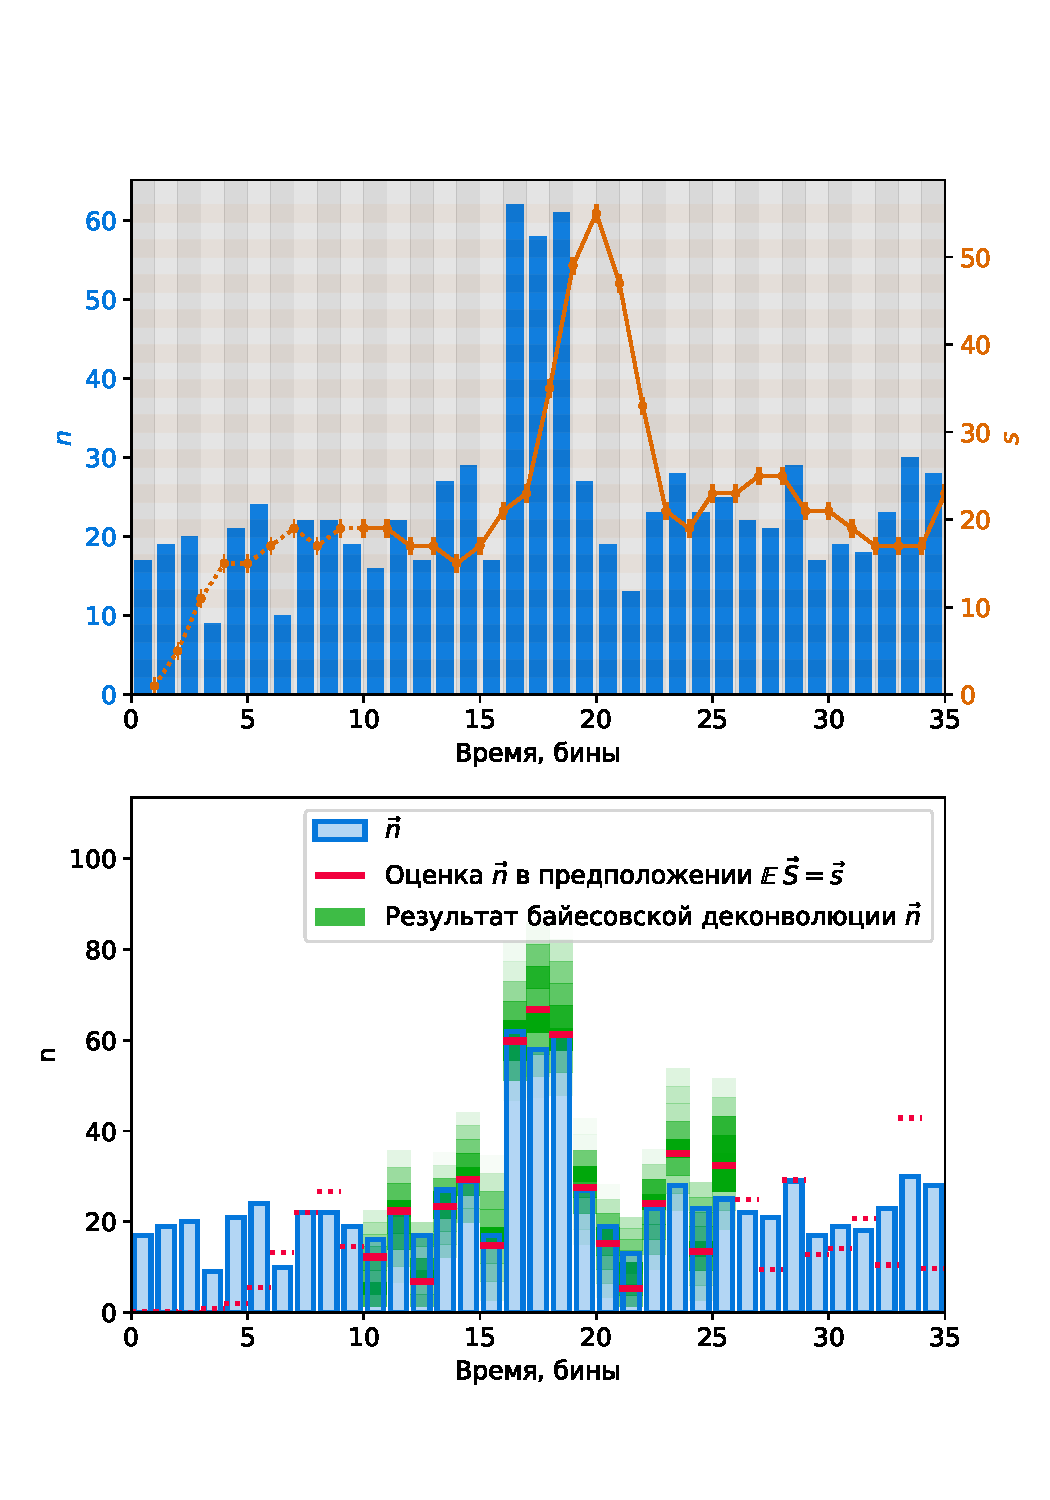
\includegraphics[width=\columnwidth]{final-problem-and-solution}
		\caption{Постановка и решение задачи байесовской деконволюции для экспериментальной РИХ с учётом погрешности измерения сигнала. В центре окна добавлена имитация пакета фотонов ШАЛ, двукратно превышающая фон в течение 3 бинов.}
		\label{pic:bayesian-deconvolution-with-experimantal-rir-and-rounding}
	\end{figure}

	\subsubsection{Каскадное сэмплирование}
	
	Полученная функция правдоподобия (\ref{eq:likelihood-with-error-uniform-error}) всё ещё требует существенного времени для вычисления. Б\'{о}льшая часть вычислений функции правдоподобия приходится на период <<разгона>> сэмплера и набора достаточного количества итераций для устойчивой оценки времени автокорреляции $\tau$ (см. параграф \ref{sec:mcmc-implementation-details}). Этот процесс можно ускорить, если инициализировать сэмплер не точками в области грубой оценки $\vec{n}$, но некоторым промежуточным распределением, близким к конечному, но более простым в получении. Такое промежуточное распределение можно получить, рассмотрев функцию правдоподобия в приближении \textit{факторизованного} многомерного нормального распределения.
	
	Если бы корреляции между элементами случайного вектора $\vec{S}$ при заданных $\vec{n}$ были бы пренебрежимо малы (то есть попарные распределения на рис. \ref{pic:s-j-pairwise-norm-assess} имели форму окружностей), вычисление функции правдоподобия даже с учётом ошибок измерения сигнала было бы гораздо проще. А именно, оно свелось бы к перемножению вероятностей получить наблюдаемое значение \textit{в каждом отсчёте}, которые в свою очередь рассчитывались бы из функции одномерного нормального распределения. С вычислительной точки зрения такой расчёт оказывается примерно в $100$ раз эффективнее, а получающееся в результате сэмплирования этой упрощенной функции правдоподобия апостериорное распределение качественно подобно истинному.

	Всё это позволяет ввести процедуру каскадного сэмплирования:
	
	\begin{enumerate}
		\item Сгенерировать длинные марковские цепи с упрощённой и вычислительно дешёвой функцией правдоподобия, тем самым получить выборку, близкую к апостериорному распределению, а также оценку времени автокорреляции $\tau$.
		\item <<Подменить>> функцию правдоподобия на истинную, и провести сравнительно короткое финальное сэмплирование, которое сойдётся уже к искомому апостериорному распределению
	\end{enumerate}

	На практике оказывается достаточным провести предварительное сэмплирование на $20000$ шагов с $256$ цепями, и затем окончательное -- всего $4000 \approxeq 2 \tau$ шагов с $128$ цепями. На рис. \ref{pic:simplified-and-true-likelihood-comparison} приведено сравнение маргинальных распределений в отдельно взятом бине после предварительного и окончательного сэмплирования. Видно постепенное уточнение оценки. С точки зрения времени вычислений предварительное сэмплирование занимает примерно в 60 раз меньше времени, несмотря на б\'{о}льшее число шагов и цепей.

	\begin{figure}
		\centering
		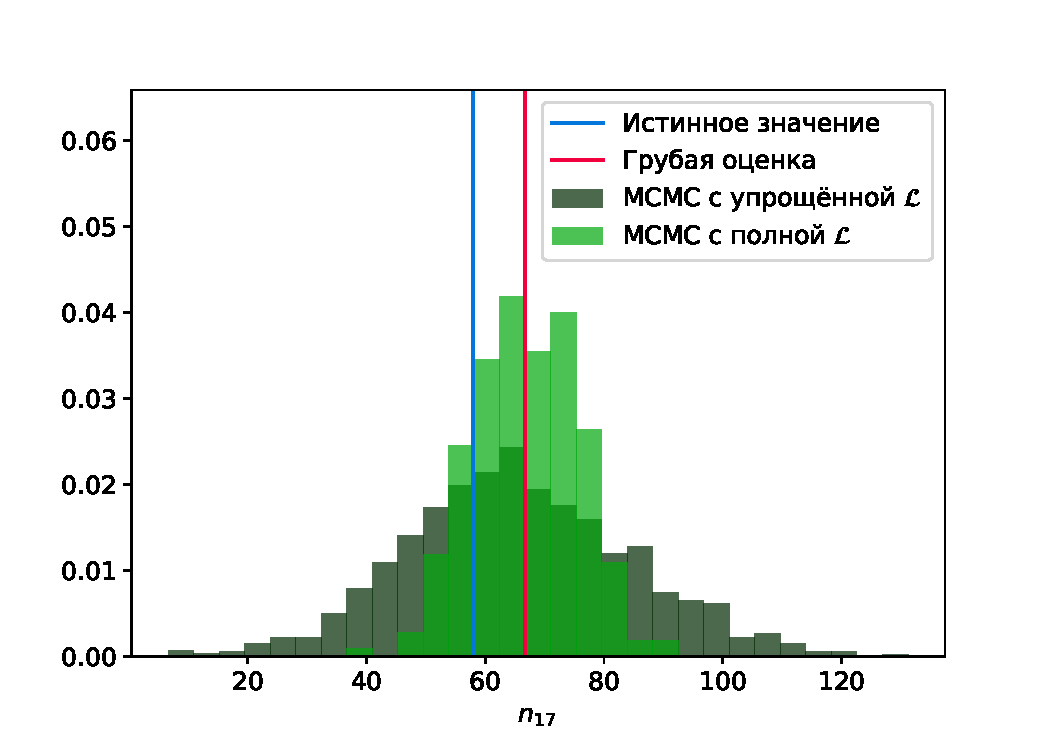
\includegraphics[width=\columnwidth]{simplified-and-true-likelihood-comparison}
		\caption{}
		\label{pic:simplified-and-true-likelihood-comparison}
	\end{figure}


	\printbibliography
	
\end{document}
